\section{Results}
\label{sec:results}





We present the results on our evaluation set of 178 GITS-Eval bugs, comprising 50 TOD bugs, 50 SAN bugs, and 78 human reported bugs. These
bugs are drawn from the Phase III bugs (see Section~\ref{sec:challengeset}) and
reflect real Google bugs that are not explicitly ruled to be outside
of the scope of Passerine capabilities (e.g., require multimedia) .


For all our experiments, we use Gemini 1.5 Pro (gemini-1.5-pro-001)~\cite{gemini1point5pro} as the LLM underlying Passerine.
We use Gemini out-of-the-box without any additional fine tuning.
LLM calls are performed with temperature = 0.2, and top\_p = 0.95, and we sample the most-likely completion.
Like many generate-and-validate APR approaches~\cite{aprbib}, we perform sampling: the agent is run for 20 (independent) trajectories, where each trajectory proceeds for a maximum of 25 steps. Code search results are limited to 5 file matches, where each 
file match can contain several matching code snippets. As discussed in Section~\ref{sec:commands},
Passerine uses the internal code search, build/test, and filesystem tools available within Google.





\subsection{Patch Correctness}
A critical measure of Passerine performance is its ability
to produce 
both plausible and valid patches. We summarize our findings in Table~\ref{tab:patch-correctness-cost-errors}.
We find that Passerine can effectively generate at
least one valid patch
for a substantial fraction of both machine-reported and
human-reported bugs.
LLM cost has not yet been optimized; we leave this to future work.
%

\begin{table}[]
\resizebox{\columnwidth}{!}{
\begin{tabular}{@{}llll@{}}
\toprule
                                                     & SAN  & TOD  & Human \\ \midrule
\% bugs with plausible patch                         & 78\% & 68\% & 25.6\%  \\
\% bugs with valid patch                             & 62\% & 24\% & 17.9\%  \\
Avg LLM calls per trajectory                         & 19.4   & 19.8 & 15.89  \\
Avg input characters per LLM call                    & 180K & 136K & 226K \\
Avg output characters per LLM call                   & 418  & 431  & 367   \\
\% trajectories that ended early due to system error & 0.7\%  & 0.2\% & 0.26\% \\ \bottomrule
\end{tabular}%

}
\caption{Summary of correctness and LLM usage for Passerine repairs.
}
\label{tab:patch-correctness-cost-errors}
\end{table}

Figure~\ref{fig:rq2-fail-to-pass} provides further
detail on patch plausibility
and validity as a function of samples. We observe
that the gap between plausibility and validity varies
by bug type, as a result of nuances in their
testing behavior. TOD bugs, which have the largest
gap, are judged
to be plausible if the test-order dependence is
removed under the original reproduction circumstances,
which specify a single ordering of tests that exhibit
test order dependency; however, this criterion may
be too lenient, and we may filter more solutions by
trying additional test orderings.
For human bugs we find that the opposite is true:
the gap between plausible and valid patch rates is small.
We observe that for these cases the plausibility criterion---the
test contained in the ground-truth commit's test file(s),
which the agent does not have access to---is a strict criterion.



















\begin{figure}
    \centering
    \begin{subfigure}{\columnwidth}
    \centering
    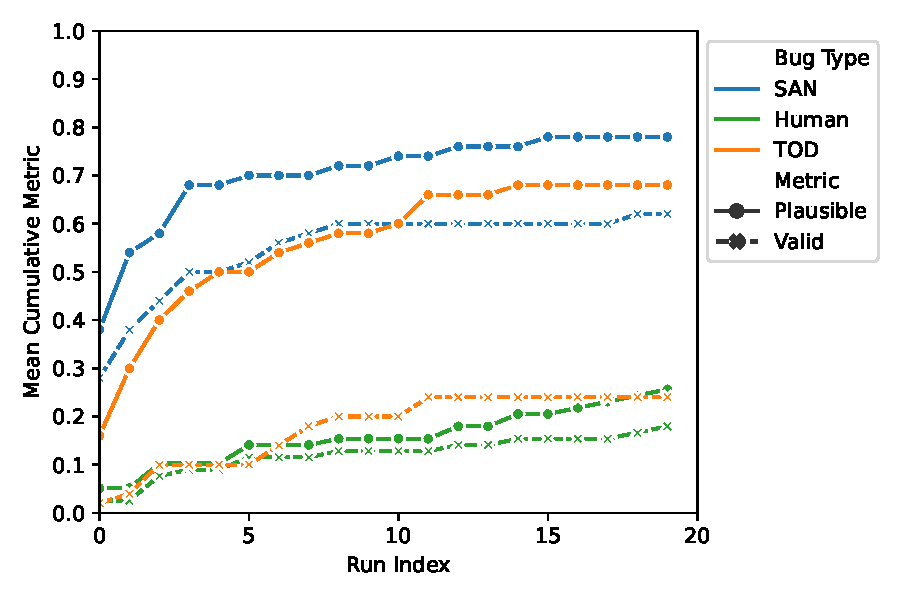
\includegraphics[width=0.8\columnwidth]{figures/mean-cumulative-stat-by-bug-type.pdf}
    \caption{
    Mean cumulative plausible and valid patch generation based on ordered trajectory samples.
    }
    \label{fig:rq2-fail-to-pass-a}
    \end{subfigure}
    ~
    \begin{subfigure}{\columnwidth}
    \centering
    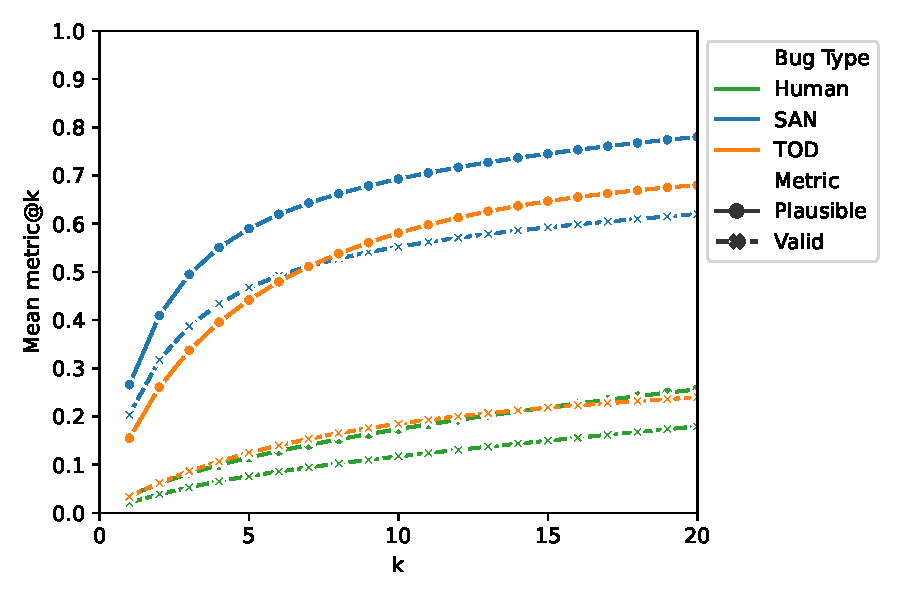
\includegraphics[width=0.8\columnwidth]{figures/mean-at-k-stats-by-bug-type.pdf}
    \caption{
    Mean plausible@k and valid@k rates, both of which are order-independent and influenced by
    fraction of samples that are plausible or valid, respectively.
    }
    \label{fig:rq2-fail-to-pass-b}
    \end{subfigure}
    \caption{
    Success metrics over 20 trajectories per bug:  Passerine can produce at least one plausible patch for 68\% of TOD bugs, 78\% of SAN bugs, and 25.6\% of Human bugs. Manual annotation shows
   24\% of TOD bugs, 62\% of SAN bugs, and  17.9\% of human-reported bugs have at least one valid patch.
}
    \label{fig:rq2-fail-to-pass}
\end{figure}








\vspace{-0.2cm}
\begin{center} 
\fbox{
\begin{minipage}[t]{0.97\linewidth}
{\bf Agent-based APR for Google bugs.} 
Our experiments show that Passerine \emph{can}
tackle bugs in Google's enterprise-scale setting, producing
plausible \emph{and} valid patches for both human-reported
and machine-reported bugs. 
\end{minipage}
}
\end{center}



\subsection{Observations}
We now share three key observations from our experiments.

\cheapsubsection{Agent strategies} 
As described in Section~\ref{sec:passerine}, 
we do not provide any high-level guidance (or restriction)
on what commands Passerine can issue or in what order.
As a result of this freedom, we observe that Passerine
can adopt different strategies for different kinds of bug reports.

Figure~\ref{fig:rq2-trajectory-comparison}
shows the frequency of commands by step index in a trajectory, grouped by bug type.
We find that early steps in human-reported bugs are typically dominated
by localization-style operations like 
\lstinline|code_search| and
\lstinline|cat|.
In contrast,
for machine-reported bugs, which, as shown in 
Figure~\ref{fig:bug-reports}, include bug reproduction
information and guidance on the kind of error,
we find that Passerine often starts by running
\lstinline|bazel| (the test building and running command). Later steps in
machine-reported bugs switch to include more edit commands.
Thus, the agent is effectively able to enter a \textit{de facto}
localization when most needed (for human-filed bugs), without
explicitly being constrained to do so, while it can also take
other actions (running tests, for machine-filed bugs) if they
might yield more useful information.
%

Additionally, we note that for SAN bugs, the first agent step
very often includes an invalid, but unnecessary, command (not in our API)
as a result of the content in the bug description, which
assumes access to \emph{all} standard Google tooling
compared to our restricted set. However, Passerine
adapts quickly and recovers in step 2, where there are no
further such commands.



\vspace{-0.2cm}
\begin{center} 
\fbox{
\begin{minipage}[t]{0.97\linewidth}
{\bf Agent strategy.} 
Despite the lack of high-level strategy guidance (e.g. there is no state machine restricting commands or per-bug-type prompt in our
implementation), Passerine adapts its strategy across bug types.
This same flexibility allows it to recover from incorrect
commands.
\end{minipage}
}
\end{center}



\begin{figure*}
    \centering
    \begin{subfigure}[b]{0.32\textwidth}
    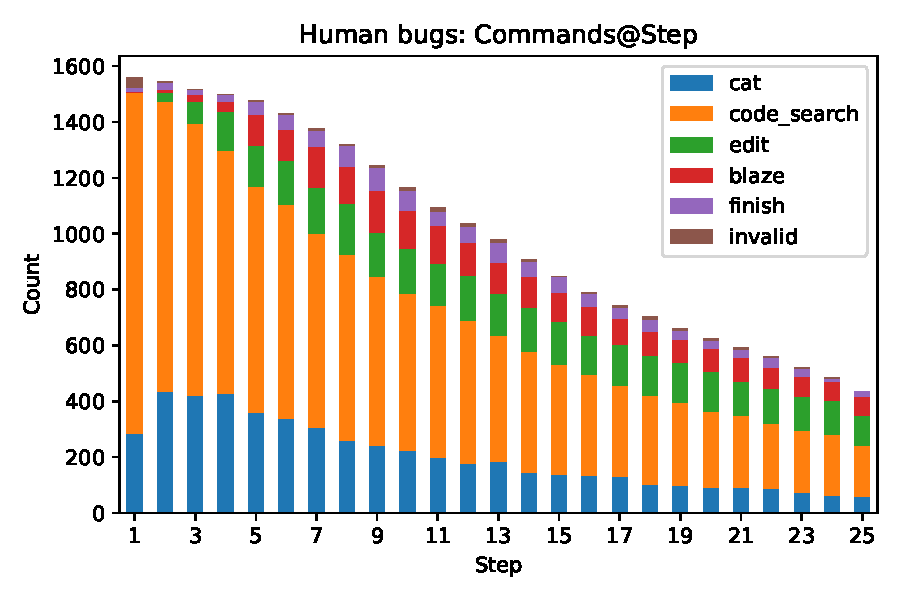
\includegraphics[width=\textwidth]{figures/human-step-command-2024-12.pdf}
    \end{subfigure}
    \begin{subfigure}[b]{0.32\textwidth}
    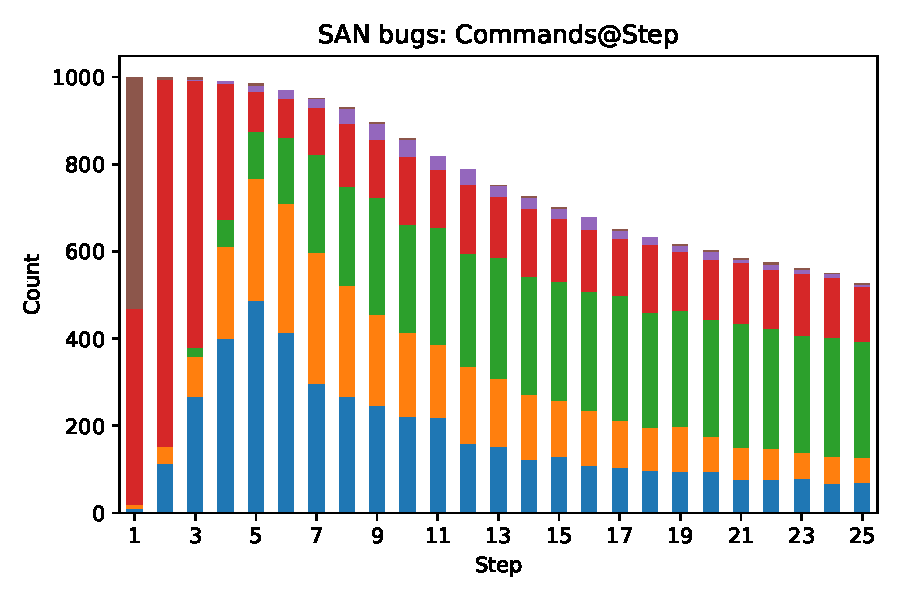
\includegraphics[width=\textwidth]{figures/chlor-step-command-2024-12.pdf}
    \end{subfigure}
    \begin{subfigure}[b]{0.32\textwidth}
    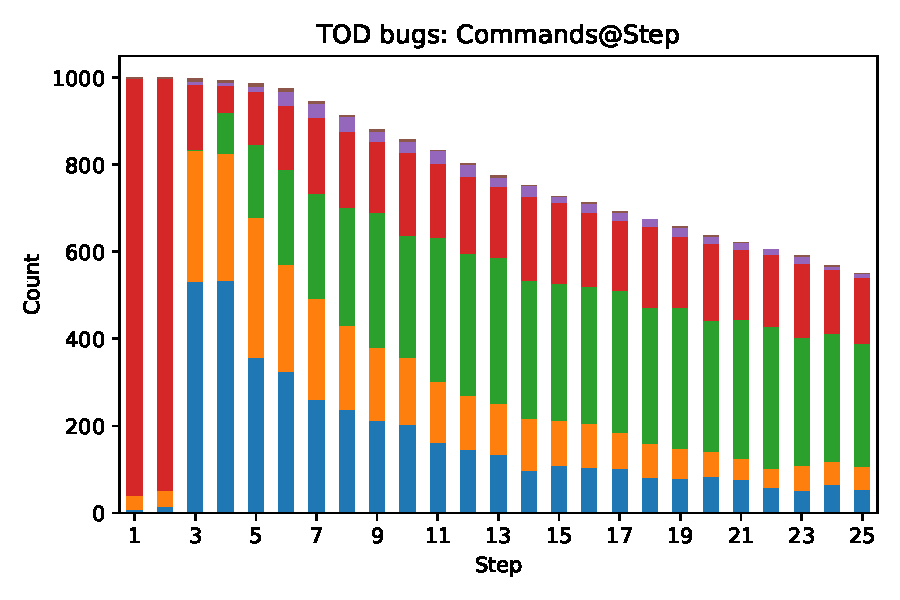
\includegraphics[width=\textwidth]{figures/testify-step-command-2024-12.pdf}
    \end{subfigure}
    \caption{
    Passerine's trajectory distributions differ substantially when applied to bugs of different types, demonstrating both the distributional differences in the information provided by each bug type and the agent's ability to adapt its behavior to the available information.
    }
    \label{fig:rq2-trajectory-comparison}
\end{figure*}






\cheapsubsection{Designing agent-informative bug reports}
To characterize
Passerine's progress on cases where the system \emph{does not}
produce a plausible patch, we consider whether the agent
at least identifies the correct files to edit. Specifically,
we compute the file-system distance between the files edited
by the agent and the ground-truth correct file locations,
where file-system distance is defined as  the distance
between two nodes (files) in an n-ary tree (file system) . 

Figure~\ref{fig:rq2-localization} shows 
that 53.8\% of machine-reported bug trajectories without a plausible
patch
edited the correct file, compared to only 3.5\% of human-reported bug trajectories without a plausible patch.
So while Passerine cannot produce a plausible patch,
it does a better job at file-level localization for machine-reported
bugs, which have rich bug reports (see Figure~\ref{fig:bug-reports}) that
include description, reproduction information, and test expectations.

The fact that an agent like Passerine can exploit this information
in bug reports, combined with the expectation that
agents will become an increasingly-common part of developer
workflows, leads us to highlight implications for researchers
and practitioners designing bug reporting platforms. Incorporating
nudges for human reporters to enrich reports
with the type of information found in machine-reported bugs
(e.g. bug reproduction guidance) can be a powerful design tool
to increase the effectiveness
of agent-based APR, allowing developers to focus their time on bugs
that are truly out of reach for current agent approaches.








\begin{figure}
    \centering
    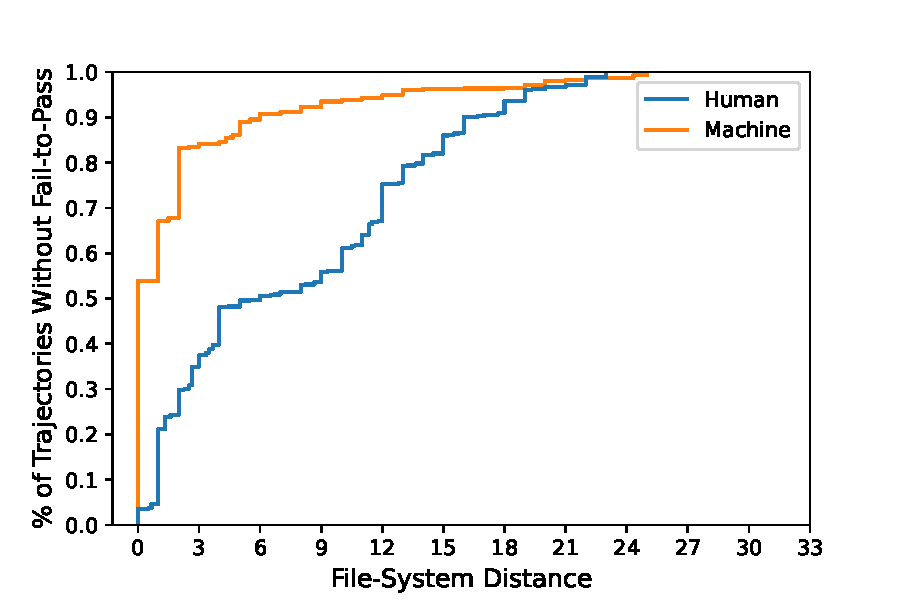
\includegraphics[width=0.7\columnwidth]{figures/localization-by-bug-type.pdf}
    \caption{Average file-system distance, defined as distance between two nodes (files) in an n-ary tree (file-system), between the agent edited files and the ground-truth files for trajectories where Passerine \emph{does not produce a fail-to-pass (i.e., not plausible)}.
    Passerine can more effectively localize machine-reported
    bugs as a result of their detailed bug descriptions.}
    \label{fig:rq2-localization}
\end{figure}

\vspace{-0.2cm}
\begin{center} 
\fbox{
\begin{minipage}[t]{0.97\linewidth}
{\bf Bug reporting.} 
Passerine can produce higher fix rates (or if it fails,
can at least localize the fault to the right file more often) when given
richer bug reports. As agent-based repair continues to gain
traction, the community should consider what nudges can
be provided to human bug reporters to increase the richness
of their issues and put them within reach of existing
agent capabilities.
\end{minipage}
}
\end{center}





\cheapsubsection{Trajectory analysis}
Performing granular inspection of Passerine
trajectories revealed interesting opportunities for additional
optimization. One such opportunity consists of identifying
(and pruning) degenerate agent trajectories, which display
clear misbehaviors. Table~\ref{tab:rq2-smells} shows 
the incidence of two basic properties that signal such
degenerate behavior. 
Trajectories without testing (\texttt{NO\_TEST\_SMELL}) suggest the agent does not
know where to start or how to confirm fixes -- this is observed in 
human bugs.
Interestingly, we also find that more subtle behaviors,
such reading a file that is already in the agent's
context (\texttt{NO\_OP\_CAT\_SMELL}), correlates with failures.
Furthermore, we note that some trajectory dynamics can reflect bug type and difficulty.
Table~\ref{tab:rq2-smells} shows that human bugs are more likely to perform
repeated consecutive searches (\texttt{CONSECUTIVE\_SEARCH}), likely due to
the lack of information contributing to localization challenges as discussed
previously. Both SAN and TOD trajectories, in contrast, are easier to localize
and the agent is more likely to perform repeated edits on the same file (\texttt{CONSECUTIVE\_EDIT}). As might be expected, both of these smells correlate
with bug difficulty and so we observe higher incidence in failing trajectories compared
to trajectories that generate a plausible patch. %



\vspace{-0.2cm}
\begin{center} 
\fbox{
\begin{minipage}[t]{0.97\linewidth}
{\bf Trajectory analysis.} 
Analyzing agent trajectories in detail, such as identifying
repeated misbehaviors, can expose opportunities for optimizations,
some of which, with little effort, could lower reviewer burden.
\end{minipage}
}
\end{center}




\begin{table}[]
\resizebox{\columnwidth}{!}{
\begin{tabular}{lrrrrrr}
\toprule
\multirow{2}{*}{Trajectory Smell} & \multicolumn{2}{c}{Human} & \multicolumn{2}{c}{SAN} & \multicolumn{2}{c}{TOD} \\ \cmidrule(l){2-7} 
 & Failing & Passing & Failing & Passing & Failing & Passing \\
\midrule
NO\_OP\_CAT\_SMELL & 0.44 & 0.22 & 0.70 & 0.53 & 0.60 & 0.54 \\
NO\_TEST\_SMELL & 0.66 & 0.13 & 0.01 & 0.00 & 0.01 & 0.00 \\
CONSECUTIVE\_SEARCH & 0.67 & 0.33 & 0.41 & 0.10 & 0.31 & 0.18 \\
CONSECUTIVE\_EDIT & 0.21 & 0.18 & 0.63 & 0.29 & 0.68 & 0.32 \\
\bottomrule
\end{tabular}
}
\caption{Smell incidence for Passerine trajectories varies across bug type and resulting patch plausibility.}
\label{tab:rq2-smells}
\end{table}











